\documentclass[a4paper]{article}
\usepackage{color}
\usepackage{tikz}
\usepackage{lipsum}
\usepackage{geometry}
\geometry{a4paper, left=3cm, top=3cm, bottom=3cm, right=3cm}
\usepackage{changepage}
\usepackage{booktabs}
\usepackage[labelfont = sc]{caption}
\DeclareCaptionFormat{mycaptionfont}{\fontsize{12}{13}\selectfont#1#2#3}
\usepackage{threeparttable}
\usepackage{graphicx}
\usepackage{ntheorem}
\usepackage{caption}
\captionsetup{format=mycaptionfont}
\usepackage{subcaption}
\theoremseparator{:}
\newtheorem{hyp}{Hypothesis}
\usetikzlibrary{shapes,decorations,arrows,calc,arrows.meta,fit,positioning}
\tikzset{
    -Latex,auto,node distance =1 cm and 1 cm,semithick,
    state/.style ={ellipse, draw, minimum width = 0.7 cm},
    point/.style = {circle, draw, inner sep=0.04cm,fill,node contents={}},
    bidirected/.style={Latex-Latex,dashed},
    el/.style = {inner sep=2pt, align=left, sloped}
}





\begin{document}
\section{Data Prep, EDA, and Theory development}
\subsection{Varaible Selection \& Explanation}
For the purpoase of analyzing the determinants of prices of home sales in the US, the followign variables were included in the analysis: 

% Table created by stargazer v.5.2.3 by Marek Hlavac, Social Policy Institute. E-mail: marek.hlavac at gmail.com
% Date and time: Wed, Sep 14, 2022 - 15:53:27
\begin{table}[!htbp] 
\begin{adjustwidth}{-1cm}{-1cm}


\begin{threeparttable}
\small
\captionsetup{font=small, justification=raggedright,singlelinecheck=false}
\caption{\textsc{Descriptive Statistics of Numeric Varaibles}}
\centering 
  \label{}   
\begin{tabular}{@{\extracolsep{5pt}}lccccccc} 
\\[-5ex]\hline 
\hline \\[-1.8ex] 
Statistic & \multicolumn{1}{c}{Mean} & \multicolumn{1}{c}{St. Dev.} & \multicolumn{1}{c}{Min} & \multicolumn{1}{c}{Pctl(25)} & \multicolumn{1}{c}{Median} & \multicolumn{1}{c}{Pctl(75)} & \multicolumn{1}{c}{Max} \\ 
\hline \\[-1.8ex] 
SalePrice & 180.921 & 79.443 & 34.900 & 129.975 & 163.000 & 214.000 & 755.000 \\ 
Lot Area & 10,516.830 & 9,981.265 & 1,300 & 7,553.5 & 9,478.5 & 11,601.5 & 215,245 \\ 
Quality & 6.099 & 1.383 & 1 & 5 & 6 & 7 & 10 \\ 
Condition & 5.575 & 1.113 & 1 & 5 & 5 & 6 & 9 \\ 
Total Living Space & 2,572.893 & 823.598 & 334 & 2,014 & 2,479 & 3,008.5 & 11,752 \\ 
Years Since Remodeling & 22.950 & 20.641 & $-$1 & 4 & 14 & 41 & 60 \\ 
\hline \\[-3.5ex] 
\end{tabular} 


\begin{tablenotes}[para,flushleft]
      \small
      \item\textit{Notes:} OLS estimates, robust standard errors in parentheses.*** p$<$0.01, ** p$<$0.05, * p$<$0.1
    \end{tablenotes}
\end{threeparttable}
\end{adjustwidth}
\end{table}

% FIGURE 
\begin{figure}
     \centering
     \begin{subfigure}[b]{0.45\textwidth}
         \centering
         \includegraphics[scale=0.3]{"/home/angelo/Documents/Uni/Courses/Advanced Statistics and programming/Assignments/assignment1/Code/h1.jpg"}
         \caption{Positive association of total Living Space \& Sale Price \& optimal line}
         \label{fig:y equals x}
     \end{subfigure}
     \hfill
     \begin{subfigure}[b]{0.45\textwidth}
         \centering
         \includegraphics[scale=0.30]{"/home/angelo/Documents/Uni/Courses/Advanced Statistics and programming/Assignments/assignment1/Code/h3.jpg"}
         \caption{Positive association of total Living Space \& Sale Price}
         \label{fig:three sin x}
     \end{subfigure}
     \hfill
     \begin{subfigure}[b]{0.45\textwidth}
         \centering
         \includegraphics[scale=0.325]{"/home/angelo/Documents/Uni/Courses/Advanced Statistics and programming/Assignments/assignment1/Code/h2.2.jpg"}
         \caption{Positive association of total Living Space \& Sale Price}
         \label{fig:five over x}
     \end{subfigure}
        \caption{Three Hypothesis Graphs displaying their repective association with the outcome variable}
        \label{fig:three graphs}
\end{figure}





















\begin{center}
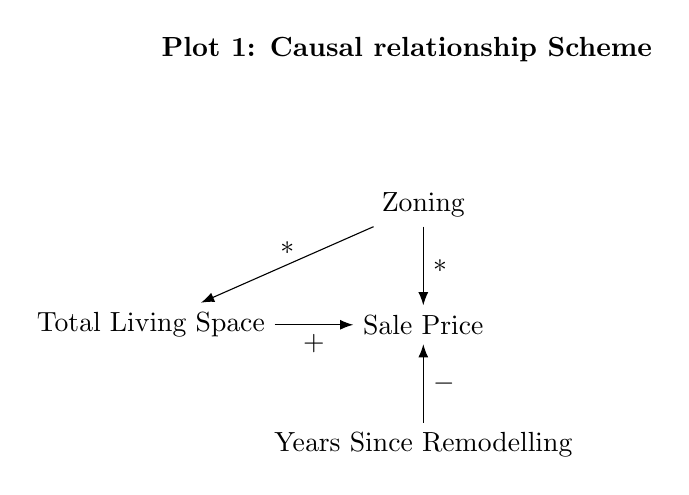
\begin{tikzpicture}
	\centering
 	\node at (3.25,3.5) {\textbf{Plot 1: Causal relationship Scheme}};
    \node (1) at (0,0) {Total Living Space};
	\node (2) [right = of 1] {Sale Price};
	\node (3) [above = of 2] {Zoning};
	\node (4) [below = of 2] {Years Since Remodelling};

	\path (1) edge node[below] {$+$} (2);
	\path (3) edge node[right] {$*$} (2);
	\path (3) edge node[above] {$*$} (1);
	\path (4) edge node[right] {$-$} (2);
	
\end{tikzpicture}
\end{center}




\end{document}
